%--------------------------------------------------------------------------------
%\documentclass{article}

\documentclass[a4paper, 12pt]{article}
\usepackage[T1]{fontenc} 
\usepackage[bf]{caption}
\usepackage{hyperref}
\usepackage[all]{hypcap}
\usepackage[utf8]{inputenc}
\usepackage{graphicx}
\usepackage[czech, english]{babel}
\selectlanguage{czech}
\usepackage{subfig}                % \subfloat
\usepackage{color}
\usepackage{url}
\inputencoding{utf8}
%\usepackage[bf]{caption2}
\usepackage{hyperref}
\usepackage[all]{hypcap}
\hypersetup{colorlinks=false, linkbordercolor=1 1 1, citebordercolor=1 1 1}
\usepackage[right]{lineno}
\renewcommand\linenumberfont{\normalfont\tiny\color{blue}}


\title{Dokumentace projektu}
\author{Vít Hodes <xhodes00@stud.fit.vutbr.cz>}
\author{Zdeněk Biberle <xbiber00@stud.fit.vutbr.cz>}
\date{\today}


%--------------------------------------------------------------------------------


\begin{document}
\selectlanguage{czech}
\maketitle

\section{Úvod}


Tato práce se zabývá implementací algoritmu Real Time Shadow of Transparent Casters Using Shadow
Volume, který jak již název naznačuje, popisuje způsob řešení stínů pomocí objemových těles, aplikovatelný i
na neuzavřené modely a tedy i obecné trojuhelníky - tzv. triangle soup. Dále algoritmus popisuje
postup tvorby stínů průhledných casterů a jejich nedokonalosti a možná řešení.

%%%%%%%%%%%%%%%%%%%%%%%%%%%%%%%%%%%%%%%%%%%%%%%%%%%%%%%%%%%%%%%%%%%%%%%%%%%%%%%%%%%%%%%%

\section{Teorie}

Tady v té kapitole je napsané jak to funguje. Ideálně nějaka ta rovnice, např. \ref{moje-rovnice}. Potom by
tady měla byt uvedena literatura, ze které bylo čerpano, například "Metody sledování paprsku jsou popsané v \cite{Byungmoon2007}"


\begin{equation}
  \label{moje-rovnice}
  c = a + b
\end{equation}

Na obrázku \ref{fig:obrazek} je ukázané jak to funguje. Nějaké schémátko pipeline..

\begin{figure}[htb]
  \centering
  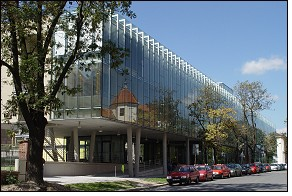
\includegraphics[width=5cm,keepaspectratio]{obrazek.jpg}
  \caption{Nějaký ten diagram, třeba převzaný }
  \label{fig:obrazek}
\end{figure}

%%%%%%%%%%%%%%%%%%%%%%%%%%%%%%%%%%%%%%%%%%%%%%%%%%%%%%%%%%%%%%%%%%%%%%%%%%%%%%%%%%%%%%%%

\section{Popis řešení­}

Tady stručně popište, jakým způsobem jste prakticky projekt řešili. Uveďte zejména použité
technologie a algoritmy. Zaměřte se hlavně na zajímavé a důležité části implementace a také na
problémy, které jste řešili. Není nutné popisovat každou třídu.

Např. uveďte, jak jste matematický popis z předchozí kapitoly implementovali prakticky.


Bylo implementováno referenční CPU řešení, které bylo p?řeváděno do compute a geometry shaderů.
Řešení se skládá prakticky ze dvou částí - spočítání objemových těles zvolenou metodou a potom
samotný proces vygenerování stínů a vykreslení.

Na začátku se předzpracují modely tak, že se odstraní duplikované vrcholy a vygenerují se nové
vertex a element vektory. Pak se vygeneruje tzv. edgeLookup vektor, ve kterém se z trojuhelníků 
vytvoří seřazená množina hran s třetím nehranovým vrcholem a id trojuhelníku. Hrany jsou seřazeny
 podle vrcholu 1, pak vrcholu 2 a nakonec podle id trojuhelníku. Toto seřazení umožňuje aby každou 
sdílenou hranu pak zpracovával jen jeden trojuhelník (ten s nejnižším id).

Implementace algoritmu se v jednotlivých implementacích příliš neliší. Ve všech případech jsou na
vstupu vrcholy modelu, element vektor definující jednotlivé trojuhelníky, edgeLookup, pozice světla a 
požadovaná délka extrudovaného stínu. V compute a geometry shaderech jsou tyto data v SSBO strukturách
(kromě pozice světla a délky stínu - ty jsou obyčejné uniformy).
 
Pro každý trojuhelník, pokud je přivrácený ke světlu, se vygeneruje nový extrudovaný o příslušnou vzdálenost
od světla. Pro každou jeho hranu se nalezne trojuhelník s nejnižším indexem, který ji obsahuje a podle
jeho orientace se nastaví multiplicita hrany (tj zda stín generuje či nikoliv).
Pokud je výsledná multiplicita nenulová, vytvoří se z příslušné hrany stěna objemového tělesa.



Postup kreslení začíná vykreslením stíněných povrchů do hloubkového bufferu, který je použitý při 
z-fail generování "stencil" textury stínů. Při z-fail algoritmu je zápis do hloubkového bufferu vypnutý
a pro každý fragment, který má hloubku větší než je aktuální v hloubkovém bufferu atomicky zapíše negativní
hodnotu své multiplicity (pro fragmenty orientované od kamery je tato hodnota ve výsledku kladná a pro
fragmenty orientované ke kameře záporná), do celočíselné "stencil" textury. Je také zapnutý early fragment test,
jinak by atomické operace prob?hly i pro fragmenty, které se budou zahazovat.

Se získanou texturou se stínem už stačí vykreslit znova stíněné předměty a pak stínící předměty bez ní.

Zajímavé řešené problémy:
Pro atomické load/store operace jsou podporovány pouze celočíselné formáty textur r32i a r32ui.
AMD má opravdu problém s přímým využitím hodnot ze SSBO pole, ale zkopírování do pomocné proměnné tento problém obejde.
Padding vstupních dat je opravdu potřeba. Dlouho nás ani nenapadlo tam hledat chybu a vůbec se tím zabývat. 

%%%%%%%%%%%%%%%%%%%%%%%%%%%%%%%%%%%%%%%%%%%%%%%%%%%%%%%%%%%%%%%%%%%%%%%%%%%%%%%%%%%%%%%%

\section{Ovládání­}

T - zapne vykreslování objemových těles
C - přepíná mezi metodami generování objemových těles
I - zapne zobrazení statistik běhu programu
R - zastaví rotaci scény
Myš - rotace okolo počátku scény
Kolečko - přiblížení/oddálení pohledu ve scén?
Esc - ukončí běh openGL programu, Enter potom celé aplikace

%%%%%%%%%%%%%%%%%%%%%%%%%%%%%%%%%%%%%%%%%%%%%%%%%%%%%%%%%%%%%%%%%%%%%%%%%%%%%%%%%%%%%%%%

\section{Vyhodnocení­}

Tady by mělo být napsané jak to funguje. Protože se jedná o počítačovou grafiku nebo 
vidění, tak by tady měl byt screenshot, ze ktereho bude poznat jak to funguje.
K tomu by měla být idealně tabulka s vyhodnocením jak přesně/rychle to funguje. 

I přes problémy s AMD hardwarem se nakonec podařilo implementaci v compute shaderech zprovoznit.
Problémy byly v paddingu vstupních struktur i samotné implementaci algoritmu, kde se počítaly
některé trojuhelníky navíc. 

----Nejaka tabulka

----Nejaky screenshot..

%%%%%%%%%%%%%%%%%%%%%%%%%%%%%%%%%%%%%%%%%%%%%%%%%%%%%%%%%%%%%%%%%%%%%%%%%%%%%%%%%%%%%%%%

\section{Závěr}

Tady by mělo být stručně napsané jak to funguje.

--znova psat jak to funguje?? 
Funguje to dle o?ekávání. Pom?rn? dob?e. Nebyl ?as.

\bibliographystyle{alpha}
\begin{flushleft}
  \bibliography{project}
\end{flushleft}

%\appendix
%\newpage
%\section{}

\end{document}
